\documentclass[11pt,a4paper]{article}
\usepackage[margin=2.5cm]{geometry}
\usepackage[utf8]{inputenc}
\usepackage[T1]{fontenc}
\usepackage{hyperref}
\renewcommand{\familydefault}{\sfdefault}
\usepackage{helvet}
\pagestyle{empty}
%\usepackage[kerning=true]{microtype}
\usepackage{parskip}
\usepackage{sansmath}
\usepackage[font={small, bf}]{caption}
\usepackage[font={small}]{subcaption}
\usepackage{graphicx}
\usepackage{multicol}
\setlength{\abovecaptionskip}{0pt}
\setlength{\floatsep}{10pt}
\setlength{\textfloatsep}{0pt}
\setlength{\intextsep}{0pt}
\setlength{\belowcaptionskip}{0pt}
\setlength{\parindent}{0ex}
\setlength{\parskip}{0pt}
% Feel free to use additional packages for glosses, figures, whatnot.

% The next bit is for reserving sufficient space for authors,
% affiliations, and e-mail address.  No need to change for initial
% anonymous version.  For the final version, replace the
% \toggletrue{anonymous} with \togglefalse{anonymous} to de-anonymize.
\usepackage{etoolbox}
\newtoggle{anonymous}
\togglefalse{anonymous}
\usepackage{ulem}
\renewcommand{\title}[1]{\textbf{#1}\\}
\newcommand{\authors}[1]{\iftoggle{anonymous}{\phantom{#1}}{#1}\\}
\newcommand{\email}[1]{\iftoggle{anonymous}{\phantom{#1}}{#1}}

\begin{document}
	


%Is there a way to give an example at the end of paragraph 1 of what a NP vs VP preposition attachment ambiguity would be, or direct readers to the example that’s on page 2 (maybe if you label the “Sentence ambiguous v unambiguous” line under the example stims for experimen 2)?



%something like “VP modifiers were preferred in the 1-referent condition (e.g. when there was a map and a manuscript to distinguish between) vs a 2-referent condition (e.g. distinguishing between two maps)- see Example Item in Experiment 2.”


	\noindent\title{Linguistic, but not visual, discourse context modulates syntactic parsing in the Maze}
	\authors{Veronica Boyce (Stanford University, vboyce@stanford.edu), Roger P. Levy (MIT)} 
	
	
	How do comprehenders  decide on parse structures when much linguistic input is temporally ambiguous?  Language is usually intended as informative and communicative, so comprehenders can rely not only on language statistics and general knowledge, but also the \textit{discourse context}, that is what entities are available in the visual or linguistic context. The use of contextual information has been most often studied with the visual world paradigm which can reveal the currently considered parse based on eye-movements\textsuperscript{1,2}. One open question is how rapidly different types of contextual information influence language processing, which can be measured using incremental processing measures to localize processing time effects. In the present work, we use the A-Maze task\textsuperscript{3,4} to explore the role of linguistic and visual discourse context in biasing syntactic attachment preferences. We describe two experiments testing NP versus VP preposition phrase attachment ambiguities in English (examples on reverse). 	\\Materials, data, code for both experiments at \url{github.com/vboyce/as-maze}.
	
	\noindent\textbf{Experiment 1: Linguistic context} We used the materials from Altmann \& Steedman (1988)\textsuperscript{5} study 2
	to see if the Maze task would reveal influences on attachment preferences based on the described context. In clause by clause SPR, A\&S found an interaction where NP modifiers were preferred in the 2-referent condition (when there were two maps to distinguish between), but VP modifiers where preferred in the 1-referent condition (when there were a map and a manuscript, see reverse for full example text). We recruited 100 participants to each read 16 of the 32 items in an A-Maze paradigm (4 per condition). For the 88 participants who had greater than 90\% overall selection accuracy, we found an expected interaction effect of 84 ms (95\% CrI 17 -- 148ms) on the disambiguating words (Table 1). Participants read words faster in the 2-referent NP and 1-referent VP conditions (Figure 1), indicating that preferred parse was influenced by whether the discourse context supported the use of a restrictive modifier. 
	
	\noindent\textbf{Experiment 2: Visual context} Visually presented context affects online sentence parsing in visual world tasks\textsuperscript{1,2}. When two objects match the noun, the following PP is interpreted as a restrictive NP-modifier, judging by eye-movements. With only one object, the PP is initially interpreted as a VP-modifier goal leading to re-analysis when the actual goal PP occurs. More recent work has shown that visual context can facilitate language processing as measured by Maze RTs\textsuperscript{6}. Here we ask if visual contexts that influence parsing in the visual world paradigm also affect Maze processing times. We used a Maze task where a context image was displayed for 5 seconds and then stayed visible as the Maze selections appeared below (example on reverse). We used a 2x2 design with 1- or 2- referent conditions in the visual context, and either ambiguous or unambiguous (``that's'' before first PP) sentences. We based our items on Weighall (2008)\textsuperscript{7}; 200 participants each saw 4 critical items (1/condition) mixed with 4 fillers. 182 participants had accuracy above 90\%. At the second preposition, there were effects of linguistic context (142ms longer RT  [-2 -- 258] in the ambiguous condition), but no effects of visual context (-27ms, [-99 -- 45]) and no interaction (-34ms, [-146 -- 86], Figure 2, Table 2). 
	
	\noindent\textbf{Discussion:} Many sources of information can constrain the meaning of incoming linguistic input, but it is unclear when different sources of information are incorporated.  Additionally, task demands may affect what information sources seem most relevant and how much information can be incorporated quickly. Here, we demonstrate that, for a prepositional phrase attachment ambiguity, linguistically presented discourse context does affect processing times during the Maze task. Co-presented visual context did not affect Maze reading times, in contrast to its effects on eye movements in visual world paradigms. This different could be due to high cognitive load from Maze and lack of task demands to closely inspect the image, or the two tasks could be querying different stages in linguistic processing and interpretation. Future work could explore whether visual discourse context influences processing times in other experimental paradigms. 
	

	
	
	\newpage
	
	
	\begin{center}\textbf{Experiment 1: Linguistic context}\end{center}
	
	\begin{minipage}{\textwidth}
		\begin{small}
			Example item:  \textit{(context sentence)} A historian was working in the British Museum holding a magnifying glass. He'd sat down to study  a map. 
			\textit{(1 or 2 referents introduced)} On his desk there was \textbf{a map} which had an appalling tear and \textbf{a  {[manuscript | map]}} which seemed in perfect condition. \textit{(a PP that resolves to NP or VP attachment, disambiguation underlined)} The historian had to study \textbf{the map with the {[\uline{appalling  tear} | 
					\uline{magnifying glass}]}} so as to value it.
				
		\end{small} 
		\medskip
	\end{minipage}
	
	\begin{minipage}{.5\textwidth}
		\captionof{figure}{Expt 1 Results}
		{	\includegraphics[width=\textwidth]{hsp_as.png}} 
		\begin{small}
			Means and bootstrapped 95\% CIs for each of the 4 conditions. Data from 88 participants who each completed 16 items. There is an interaction between the context and what the PP modifies. 
			
		\end{small}
		
	\end{minipage}
	~~
	\begin{minipage}{.45\textwidth}
		\begin{small}
			\captionof{table}{Expt 1  model coefficients}
			\begin{tabular}{|l|l|l|}
				\hline
				Term & Est. & 95\% CrI \\
				\hline
				Intercept & 995 ms & [943 -- 1046] \\
				Type (VP) & -73 ms & [-134 -- -11] \\
				Context (2-referent) & 22 ms & [-13 -- 59] \\
				Type x Context & 84 ms  & [17 -- 148] \\
				\hline
			\end{tabular}
			\vspace{2pt}
			
			Model: \textit{RT $\sim$ type $\times$ context + (type $\times$ context | item ) + (type $\times$ context | subject) } 
			Fit to reading times on the disambiguating words for correct responses only. Type and context were sum coded (VP, 2-referent coded as +.5; NP, 1-referent as -.5) and weakly regularizing priors were used. 
			
		\end{small}
		
	\end{minipage}
	
	\smallskip
	\rule{\textwidth}{1pt}
	\begin{center}\textbf{Experiment 2: Visual context}\end{center}
	
	\begin{minipage}{.3\textwidth}
		\begin{small}Example item:\\\textit{Visual context:} \\ (seen for 5 seconds before starting sentence) 
		
		\end{small}
	\end{minipage}	~~~
	\begin{minipage}{.3\textwidth}
		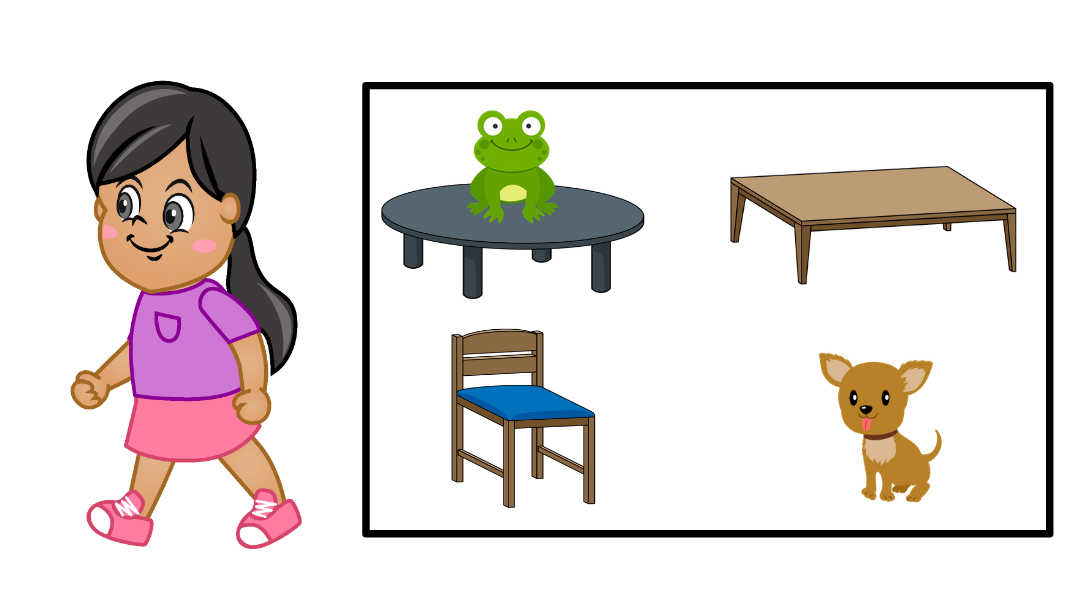
\includegraphics[width=.75\textwidth]{frog_1.png}		\begin{small}\\
			1-referent (frog and dog) 
			
			\end{small}
		
	\end{minipage}
	~~~
	\begin{minipage}{.3\textwidth}	
		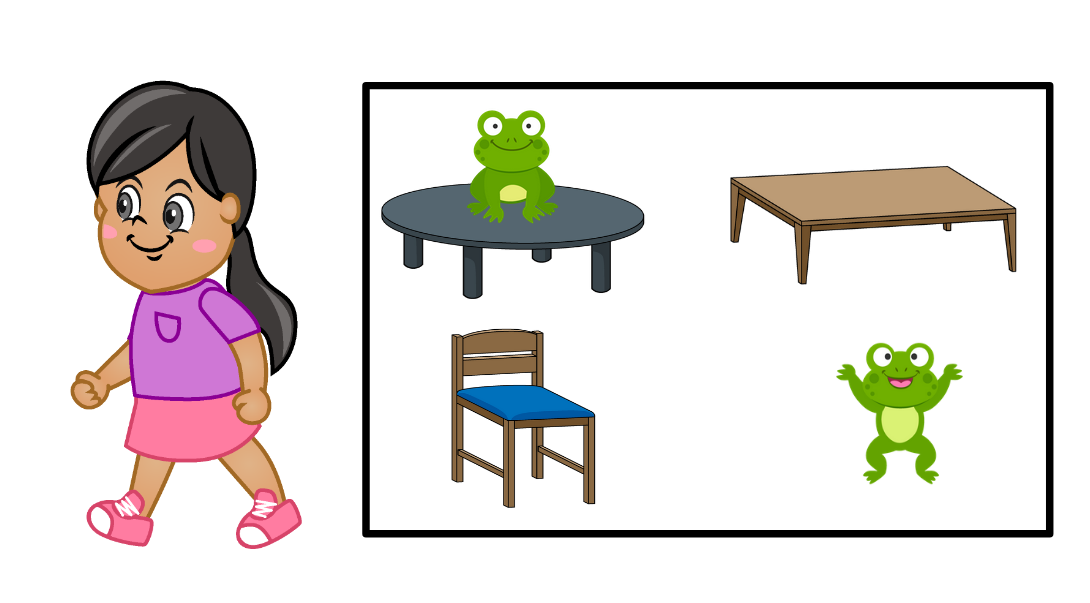
\includegraphics[width=.75\textwidth]{frog_2.png}
		\begin{small}\\ 2-referent (2 frogs) 
		
		\end{small}
		
	\end{minipage}
	
	\begin{minipage}{\textwidth}
		\begin{small}
			\textit{Sentence (ambiguous v unambiguous):} The girl will put the frog [\textbf{that's}] on the table on the chair.
			
		\end{small}
		
	\end{minipage}
	
	\vspace{10pt}
	\begin{minipage}{.65\textwidth}
		\captionof{figure}{Expt 2 Results}
		{	\includegraphics[width=\textwidth]{hsp_kpath.png}} 
		
	\end{minipage}
	~~~
	\begin{minipage}{.3\textwidth}		\begin{small}
			
			Estimate and bootstrapped 95\% CI for each of the 4 conditions. The second preposition (boxed) is the critical position. Data from 182 participants who each saw 4 critical items. There is a main effect of sentence type, where ambiguous sentences have a longer RTs on the second PP, but no interaction with visual context. 
			
		\end{small}
	\end{minipage}
	
	\begin{minipage}{.48\textwidth}
		\begin{small}
			\captionof{table}{Expt 2 model coefficients}
			\begin{tabular}{|l|l|l|}
				\hline
				Term & Est. & 95\% CrI \\
				\hline
				Intercept & 931 ms & [811 -- 1041] \\
				Type (Ambiguous) & 142 ms & [-2 -- 258] \\
				Context (2-referent) & -27 ms & [-99 -- 45] \\
				Type x Context & -34 ms  & [-146 -- 86] \\
				\hline
			\end{tabular}
		\end{small}
	\end{minipage}
	~~
	\begin{minipage} {.5\textwidth}\begin{small}
			Model: \textit{RT $\sim$ type $\times$ context + (type $\times$ context | item) + (type $\times$ context | subject)}
			Fit to reading times on the second preposition for correct responses only. Type and context were sum coded (Ambiguous, 2-referent coded as +.5; unambiguous, 1-referent as -.5) and weakly regularizing priors were used. 
			
		\end{small}
	\end{minipage}
	
	\vspace{5pt}
	\rule{\textwidth}{1pt}
	
	
	\begin{minipage}{\textwidth}
		\vspace{5pt}
		\begin{small} \textbf{References:} $\bullet$	
			1. Tanenhaus et al. Science, 1995. $\bullet$
			2. Trueswell et al. Cognition, 1999. $\bullet$
			3. Boyce, Futrell, Levy. JML, 2020. $\bullet$
			4. Boyce, Levy. Glossa Psycholinguistics, 2023. $\bullet$
			5. Altmann, Steedman. Cognition, 1988. $\bullet$
			6. Pushpita \& Levy. CoNLL, 2024. $\bullet$
			7. Weighall. J Exp Child Psych, 2008.
		\end{small}
	\end{minipage}
	
	
\end{document}